\chapter{Data and Processing Volume Estimates: (Schellman, Junk, Muether)}
\label{ch:est}

In this chapter we will describe the assumptions that go into a bottoms-up estimate of data volumes and describe possible methods of reducing the total volumes while retaining physics capabilities. 

%%%%%%%%%%%%%%%%%%%%%%%%%%%%%%%%
\section{Assumptions}
\label{sec:est:assume}  %% fix label according to section

\subsection{Raw data assumptions}
DUNE's detectors will produce information from a variety of technologies.  We anticipate that raw data volumes will be dominated by the digitized waveforms from liquid argon detectors and, to a lesser extent, photon detectors, in \dword{pd}, the \dword{fd} and the \dword{nd}.  
These raw data volumes can be reduced by the \dword{daq} system by several means.


\begin{itemize} 
\item triggered readout of particular time slices
\item triggered readout of particular geographic regions
\item lossless zero suppression
\item lossy zero suppression
\item hardware pattern recognition
\end{itemize}

Overall, we assume that the above methods can reduce data volumes from the hundreds of Exabytes that would be produced by continuous readout to a manageable 30 PB/year. 

\subsection{Derived data assumptions}


 \begin{dunetable}[Data Retention Policies]{llrrrr}{tab:est:retention}
{Retention policies by data tier}
Tier&Description&Tape copies& Lifetime &Disk Copies& Lifetime\\
Raw & Physics data& 2 & indefinitely & 1 & 1 year\\
Test & test and commissioning & 1 &6 months &1 & 6 months \\
Hits & reconstructed hits & 1 & 10 years & 1 & 1 month \\
Reco & pattern recognition &1 & 10 years & 2 & 2 years\\
\end{dunetable}

\section{ProtoDUNE}
\label{sec:est:ProtoDUNE}  

Our estimates  are largely based on our experience with the protoDUNE detectors which ran at CERN in late 2018.  The \dword{pdsp} detector read out 6 \dwords{apa} and a mix of photon detectors while the first far detector module will have 150 \dwords{apa} and photon detectors based on the \dword{arapuca} technology.  Data rates and assumptions for protoDUNE have been documented in \href{docdb:20515}{https://docs.dunescience.org/cgi-bin/private/ShowDocument?docid=20515}.  Table \ref{tab:est:usefulpd} provides useful quantities for data volumes derived from the ProtoDUNE experience. 

 \begin{dunetable}[Useful quantities for computing far detector data volumes]{lrr}{tab:est:usefulpd}
{Useful quantities for computing estimates for \dword{sp}
readout.   }%\rowtitlestyle
Quantity&Value&Explanation\\
\toprowrule
%{\bf Far Detector Beam:}\\ \colhline
Number of channels/APA&2,560&\\
Readout time & 3 ms&\\
\# of time slices & 6000&\\
Single APA readout &23 MB& Uncompressed  estimate\\ \colhline
APAs & 6 &\\
Full detector readout &178 MB& Uncompressed real \\ \colhline
Full detector readout &71 MB& Compressed real \\ \colhline
Effective compression factor &2.5&\\ \colhline
Beam rep. rate&4.5 Hz&Average\\ \colhline
Hit reconstruction time CPU time/APA& 30 sec&from MC/ProtoDUNE\\ \colhline
Pattern recognition time CPU time event & 400 sec&from MC/ProtoDUNE\\ \colhline
Simulation time CPU time event & 2700 sec&from MC/ProtoDUNE\\ \colhline
Memory footprint/APA&0.5-1GB&ProtoDUNE experience\\ \colhline
\end{dunetable}

 

For example, uncompressed single phase data from ProtoDUNE-SP were observed to be around 178 MB in size, which is the amount expected for the number  of TPC channels read + a 20\% overhead for other detectors and headers.  Compressed SP data averages 71 MB, consistent with compression by a factor of 2.5.  

Dual phase data includes 2 CRPs for the 2019 run.  Observed data size without compression  was 110MB.  %Numbers for 2018 and 2019 have been 

For the far detector with APA's we assume 






[DUNE-doc-20515-v6]

\section{FD}
\label{sec:est:FD}  

For far detector data volumes, we use our \dword{pdsp} experience and assume that raw data sizes and hit finding CPU times scale with the number of \dwords{apa} while pattern recognition and simulation times scale with the number of interactions. 

 \begin{dunetable}[Useful quantities for computing \dshort{sp}
estimates]{lrr}{tab:est:usefulfd}
{Useful quantities for computing estimates for \dword{sp}
readout.}%\rowtitlestyle
Quantity&Value&Explanation\\
\toprowrule
{\bf Far Detector Beam:}\\ \colhline
Single APA readout &41.5 MB& Uncompressed 5.4 ms\\ \colhline
APAs per module& 150&\\
Compression factor &2.5 &\\
One full module readout &6.22  GB& Uncompressed 5.4 ms\\ \colhline
One full module readout &2.49  GB& Compressed 5.4 ms\\ \colhline
Beam rep. rate&\beamreprate&Untriggered\\ \colhline
Hit finding CPU time/APA&30 sec&from MC/ProtoDUNE\\ \colhline
Pattern recognition CPU time/event&400 sec&from MC/ProtoDUNE\\ \colhline
Simulation time CPU time event & 2700 sec&from MC/ProtoDUNE\\ \colhline
Memory footprint/APA&0.5-1GB&ProtoDUNE experience\\ \colhline
{\bf Supernova:}\\ \colhline
Single channel readout &300 MB& Uncompressed 100 s\\ \colhline
Four module readout& 460 TB& Uncompressed 100 s\\ \colhline
Four module readout& 184 TB& Compressed 100 s\\ \colhline
Trigger rate&1  per month&(assumption)\\
\end{dunetable}


DUNE \href{docdb:14893}{https://docs.dunescience.org/cgi-bin/private/ShowDocument?docid=14983} describes the expected event rates for various signatures in a \dword{fd} module.  These can be combined with the above numbers to provide  the integrated data estimates shown in table \ref{tab:estfdrates}. 

 \begin{dunetable}
 [Far detector data volumes] {|l |r r r |}{tab:est:fdrates}
{Data sizes and rates for different processes in each far detector module.  Uncompressed data sizes are given. As readouts will be self-triggering an extended 5.4 ms readout window is used instead of the 3ms for the triggered \dword{pdsp} runs.  We assume beam uptime of 50\% and 100\% uptime for non-beam science. These numbers are derived from references \cite{bib:docdb16028} and \cite{bib:docdb14983}.}
%\rowtitlestyle
%Quantity&Value&Explanation\\
%\toprowrule
%\begin{tabular}{|l |r r r |}
%\hline
Process & Rate/module & \qquad size/instance &\qquad  size/module/year\\
\hline
Beam event & 41/day & 6 GB&47 TB/year\\
Cosmic rays &4,500/day&  6 GB& 9.7 PB/year\\
Supernova trigger& 1/month& 115 TB& 1.4 PB/year\\
Calibrations&2/year&750 TB& 1.5 PB/year\\
\hline 
Total& & &12.9 PB/year\\
\end{dunetable}%



\section{ND}
\label{sec:est:ND}  

This section is based on the estimates provided in the Near Detector CDR [DUNE-doc-21267-v2]

\section{Summary}
\label{sec:est:volumes}

Given the above estimates we can  estimate total disk and CPU needs every year.

Figure \ref{fig:est:events} shows the estimate number of events/year for each detector type.  

\begin{dunefigure}
[Event estimates]
{fig:est:events}
{Number of events per year used in data volume estimates. }
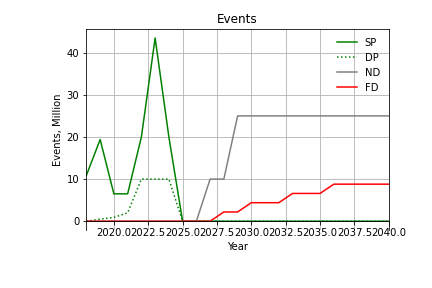
\includegraphics[width=0.8\textwidth]{IntroFigures/Events.png}
\end{dunefigure}

CPU and size/readout are drawn from the above estimates. We then make the following assumptions about data sizes and retention.  
Figures \ref{fig:est:disk,fig:est:tape,fig:est:cores} illustrate the estimated storage and CPU needs through 2030.  In the early years, \dword{pd} and \dword{nd} prototype tests dominate while commissioning and operation of the first (and second) \dword{fd} and the \dword{nd} become important after 2026. 

\begin{itemize}
\item Two copies of raw data are retained indefinitely
\item Commissioning data is marked test and one copy is retained on disk for 6 months. 
\item Reconstruction is performed on the full data sample once/year and 2 copies are retained on disk for 2 years.  
\item Analysis includes calibration and is  equivalent to reconstruction but produces smaller outputs. 
\end{itemize}

\begin{dunefigure}
[Disk estimates]
{fig:est:disk}
{Estimated size of various samples in PB. This estimate includes retention policies and multiple copies.}
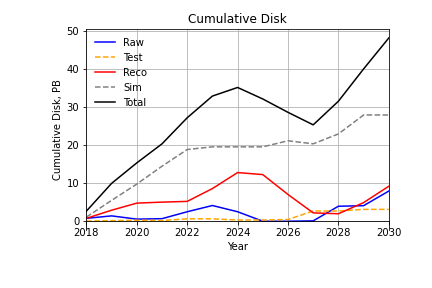
\includegraphics[width=0.8\textwidth]{IntroFigures/Cumulative-Disk.png}
\end{dunefigure}

\begin{dunefigure}
[Tape estimates]
{fig:est:tape}
{Estimated size of various samples in PB. This estimate includes retention policies and multiple copies.}
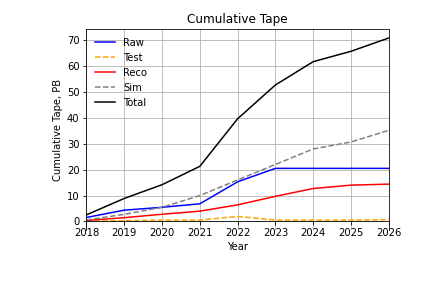
\includegraphics[width=0.8\textwidth]{IntroFigures/Cumulative-Tape.png}
\end{dunefigure}

\begin{dunefigure}
[Tape estimates]
{fig:est:cores}
{Estimated CPU needs for  various samples.  The units are present day cores assuming 70\% efficiency.}
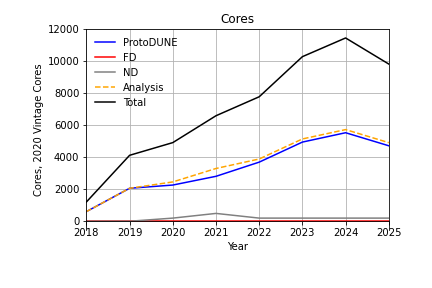
\includegraphics[width=0.8\textwidth]{IntroFigures/Cores.png}
\end{dunefigure}